\chapter{Proofs for \cref{chapter_bipartite_tournaments}}
\label{chapter_tourn_proofs}

\section{Proof of \Cref{tourn_result_mle_hamming}}

The proof of \Cref{tourn_result_mle_hamming} requires a lemma of its own.

\begin{lemma}
   \label{tourn_result_probexpression}

   Let $K$ be an $m \times n$ tournament, $\bm{\alpha} \in [0,1]^2$ and
   $\theta \in \Theta_{m,n}$. Then
   \begin{equation*}
      \begin{split}
          P_{\bm{\alpha}}(K \mid \theta)
          =
          \prod_{a \in A}
            &\alpha_+^{|K(a) \setminus K_\theta(a)|}
            (1 - \alpha_-)^{|K(a) \cap K_\theta(a)|}
            \\
            &\quad (1 - \alpha_+)^{|B \setminus (K(a) \cup K_\theta(a))|}
            \alpha_-^{|K_\theta(a) \setminus K(a)|}
      \end{split}
   \end{equation*}
\end{lemma}

\begin{proof}
    Write $p_{ab,K}$ for $P_{\bm{\alpha}}(X_{ab} = K_{ab} \mid \theta)$.
    Expanding the product in \cref{tourn_def_probdist}, we have
    \[
       P_{\bm{\alpha}}(K \mid \theta)
       = \prod_{a \in A}{\prod_{b \in B}{p_{ab,K}}}
    \]

    Let $a \in A$. Note that $B$ can be written as the disjoint
    union $B = B_1 \cup B_2 \cup B_3 \cup B_4$, where
    \[
       \begin{aligned}
          B_1 &= K(a) \setminus K_\theta(a) \\
          B_2 &= K(a) \cap K_\theta(a) \\
          B_3 &= B \setminus (K(a) \cup K_\theta(a)) \\
          B_4 &= K_\theta(a) \setminus K(a)
       \end{aligned}
    \]
    Recall that $b \in K_\theta(a)$ iff $x_a \ge y_b$
    (where $\theta = \tuple{\bm{x}, \bm{y}}$).  It follows that

    \begin{itemize}
        \item $b \in B_1$ iff $K_{ab} = 1$ and $x_a < y_b$
        \item $b \in B_2$ iff $K_{ab} = 1$ and $x_a \ge y_b$
        \item $b \in B_3$ iff $K_{ab} = 0$ and $x_a < y_b$
        \item $b \in B_4$ iff $K_{ab} = 0$ and $x_a \ge y_b$
    \end{itemize}

    Note that this correspond exactly to the four cases in
    \labelcref{tourn_eqn_probdist_random_var_one} and
    \labelcref{tourn_eqn_probdist_random_var_zero} which define $p_{ab, K}$; we have
    \[
        p_{ab,K} = \begin{cases}
            \alpha_+,& b \in B_1 \\
            1 - \alpha_-,& b \in B_2 \\
            1 - \alpha_+,& b \in B_3 \\
            \alpha_-,& b \in B_4
        \end{cases}
    \]
    Consequently
    \[
       \begin{aligned}
           \prod_{b \in B}{p_{ab,K}}
           &=
               \left(\prod_{b \in B_1}{\alpha_+}\right)
               \left(\prod_{b \in B_2}{(1-\alpha_-)}\right)
               \left(\prod_{b \in B_3}{(1-\alpha_+)}\right)
               \left(\prod_{b \in B_4}{\alpha_-}\right)
           \\
           &= \alpha_+^{|B_1|} (1-\alpha_-)^{|B_2|} (1-\alpha_+)^{|B_3|}
              \alpha_-^{|B_4|} \\
           &= \alpha_+^{|K(a) \setminus K_\theta(a)|}
              (1-\alpha_-)^{|K(a) \cap K_\theta(a)|}
              \\
           &\quad \quad (1-\alpha_+)^{|B \setminus (K(a) \cup K_\theta(a))|}
              \alpha_-^{|K_\theta(a) \setminus K(a)|}
       \end{aligned}
    \]
    Taking the product over all $a \in A$ we reach the desired
    expression for $P_{\bm{\alpha}}(K \mid \theta)$.
\end{proof}

\begin{proof}[Proof of \Cref{tourn_result_mle_hamming}]
    Let $\theta \in \Theta_{m,n}$. From \cref{tourn_result_probexpression} we get
    \[
       \begin{aligned}
       P_{\bm{\alpha}}(K \mid \theta)
       = \prod_{a \in A}
            &\beta^{
              |K(a) \setminus K_\theta(a)| + |K_\theta(a) \setminus K(a)|
            }
            \\
            &\quad (1 - \beta)^{
              |K(a) \cap K_\theta(a)|
              + |B \setminus (K(a) \cup K_\theta(a))|
            }
       \end{aligned}
    \]
    Note that
    \[
       |K(a) \setminus K_\theta(a)| + |K_\theta(a) \setminus K(a)|
       =
       |K(a) \symdiff K_\theta(a)|
    \]
    \[
       |K(a) \cap K_\theta(a)|
       + |B \setminus (K(a) \cup K_\theta(a))|
       =
       |B| - |K(a) \symdiff K_\theta(a)|
    \]
    and so
    \[
       \begin{aligned}
           P_{\bm{\alpha}}(K \mid \theta)
           &= \prod_{a \in A}{
                \beta^{
                  |K(a) \symdiff K_\theta(a)|
                }
                (1 - \beta)^{
                  |B| - |K(a) \symdiff K_\theta(a)|
                }
           } \\
           &= \prod_{a \in A}{
                \left(
                  \frac{\beta}{1 - \beta}
                \right)^{
                  |K(a) \symdiff K_\theta(a)|
                }
                (1 - \beta)^{|B|}
           } \\
           &= \underbrace{
                (1 - \beta)^{|A| \cdot |B|}
              }_{=c}
               \prod_{a \in A}{
                \left(
                  \frac{\beta}{1 - \beta}
                \right)^{
                  |K(a) \symdiff K_\theta(a)|
                }
           } \\
           &= c
              \prod_{a \in A}{
               \left(
                 \frac{\beta}{1 - \beta}
               \right)^{
                 |K(a) \symdiff K_\theta(a)|
               }
           }
       \end{aligned}
    \]
    where $c$ is a positive constant that does not depend on $\theta$. Now,
    $P_{\bm{\alpha}}(K \mid \theta)$ is positive, and is maximal when its
    logarithm is. We have
    \[
       \begin{aligned}
           \log{P_{\bm{\alpha}}(K \mid \theta)}
           &=
              \log{c}
              + \sum_{a \in A}{
                  |K(a) \symdiff K_\theta(a)|
                  \log{\left(\frac{\beta}{1 - \beta}\right)}
              } \\
           &=
              \log{c}
              +
              \log{\left(\frac{\beta}{1 - \beta}\right)}
              \sum_{a \in A}{
                  |K(a) \symdiff K_\theta(a)|
              } \\
           &=
              \log{c}
              +
              \log{\left(\frac{\beta}{1 - \beta}\right)}
              d(K, K_\theta)
       \end{aligned}
    \]
    Noting that $\beta < 1/2$ implies $\log{\left(\frac{\beta}{1 -
    \beta}\right)} < 0$, it follows that for any $\theta, \theta' \in
    \Theta_{m,n}$:
    \[
       \begin{aligned}
          P_{\bm{\alpha}}(K \mid \theta)
              \ge P_{\bm{\alpha}}(K \mid \theta')
          &\iff \log{P_{\bm{\alpha}}(K \mid \theta)}
              - \log{P_{\bm{\alpha}}(K \mid \theta')} \ge 0 \\
          &\iff \underbrace{\log{\left(\frac{\beta}{1 - \beta}\right)}}_{<0}
              \left[
                d(K, K_{\theta}) - d(K, K_{\theta'})
              \right]
              \ge 0 \\
          &\iff d(K, K_{\theta}) \le d(K, K_{\theta'})
       \end{aligned}
    \]
    which proves the result.
\end{proof}

\section{Proof of \Cref{tourn_result_chain_iff_ktheta}}

We need a preliminary result.

\begin{lemma}
   \label{tourn_result_ktheta_ordering}

   Let $\theta = \tuple{\bm{x}, \bm{y}} \in \Theta_{m,n}$. Then for all
   $a, a' \in A$ and $b, b' \in B$:

   \begin{enumerate}
       \item $K_\theta(a) \subseteq K_\theta(a')$ iff $x_a \le
             x_{a'}$
       \item $K_\theta^{-1}(b) \supseteq K_\theta^{-1}(b')$ iff $y_b
             \le y_{b'}$.
   \end{enumerate}
\end{lemma}

\begin{proof}

    We prove (1); (2) is shown similarly. Let $a, a' \in A$. First suppose $x_a
    \le x_{a'}$. Let $b \in K_\theta(a)$. Then $y_b \le x_a \le x_{a'}$, so $b
    \in K_\theta(a')$ also. This shows $K_\theta(a) \subseteq K_\theta(a')$.

    Now suppose $K_\theta(a) \subseteq K_\theta(a')$. For the sake of
    contradiction, suppose $x_a > x_{a'}$. By \labelcref{tourn_eqn_state_condition_a}
    in the definition of a state (\cref{tourn_def_stateworld}), there is $b \in B$
    such that $x_{a'} < y_b \le x_{a}$. But this means $b \in K_\theta(a)
    \setminus K_\theta(a')$, which contradicts $K_\theta(a) \subseteq
    K_\theta(a')$. Thus (1) is proved.
\end{proof}

\begin{proof}[Proof of \Cref{tourn_result_chain_iff_ktheta}]
    The ``if'' direction follows from \cref{tourn_result_ktheta_ordering} part (1):
    if $\theta = \tuple{\bm{x}, \bm{y}}$ and $a, a' \in A$ then
    either $x_a \le x_{a'}$ -- in which case $K_\theta(a)
    \subseteq K_\theta(a')$ -- or $x_{a'} < x_a$ -- in
    which case $K_\theta(a') \subseteq K_\theta(a)$. Therefore $K_\theta$ has
    the chain property.

    For the ``only if'' direction, suppose $K$ has the chain property.
    Define $\theta = \tuple{\bm{x}, \bm{y}}$ by

    \[
       \begin{aligned}
           x_a &= |\{a' \in A \mid K(a') \subseteq K(a)\}| \\
           y_b &= \begin{cases}
              \min\{x_a \mid a \in K^{-1}(b)\}
                  ,& K^{-1}(b) \ne \emptyset \\
              1 + |A|,& K^{-1}(b) = \emptyset
           \end{cases}
       \end{aligned}
    \]

    It is easily that since the neighbourhood-subset relation ${\anle_K}$ is a
    total preorder, we have $K(a) \subseteq K(a')$ if and only if $x_a \le
    x_{a'}$.  First we show that $K_\theta = K$ by showing that $K_{ab} = 1$ if
    and only if $[K_\theta]_{ab} = 1$. Suppose $K_{ab} = 1$. Then $a \in
    K^{-1}(b)$, so $y_b = \min\{x_{a'} \mid a' \in K^{-1}(b)\} \le x_a$ and
    consequently $[K_\theta]_{ab} = 1$.

    Now suppose $[K_\theta]_{ab} = 1$. Then $x_a \ge y_b$.  We must have
    $K^{-1}(b) \ne \emptyset$; otherwise $y_b = 1 + |A|
    > |A| \ge x_a$. We can therefore take $\hat{a} \in \argmin_{a'
    \in K^{-1}(b)}{x_{a'}}$. By definition of $y_b$, $x_{\hat{a}} = y_b \le
    x_a$. But $x_{\hat{a}} \le x_a$ implies $K(\hat{a}) \subseteq K(a)$; since
    $\hat{a} \in K^{-1}(b)$ this gives $b \in K(\hat{a})$ and $b \in K(a)$,
    i.e. $K_{ab} = 1$. This completes the claim that $K = K_\theta$.

    It only remains to show that $\theta$ satisfies conditions
    \labelcref{tourn_eqn_state_condition_a} and \labelcref{tourn_eqn_state_condition_b} of
    \cref{tourn_def_stateworld}. For \labelcref{tourn_eqn_state_condition_a}, suppose $x_a
    < x_{a'}$. Then $K(a) \subset K(a')$, i.e there is $b \in K(a') \setminus
    K(a) = K_\theta(a') \setminus K_\theta(a)$. But $b \in K_\theta(a')$ gives
    $y_b \le x_{a'}$, and $b \not\in K_\theta(a)$ gives $x_a < y_b$; this shows
    that \labelcref{tourn_eqn_state_condition_a} holds.

    For \labelcref{tourn_eqn_state_condition_b}, suppose $y_b < y_{b'}$. Clearly
    $K^{-1}(b) \ne \emptyset$ (otherwise $y_b = 1 + |A|$ is maximal). Thus
    there is $a \in K^{-1}(b)$ such that $y_b = x_a$. This of course means $x_a
    < y_{b'}$; in particular we have $y_b \le x_a < y_{b'}$ as required for
    \labelcref{tourn_eqn_state_condition_b}.

    We have shown that $K = K_\theta$ and that $\theta \in \Theta_{m,n}$, and the
    proof is complete.
\end{proof}

\section{Proof of \Cref{tourn_result_mle_iff_chainmin_operator}}

\begin{proof}

    First we show that for any $m, n \in \N$ and any $m \times n$ tournament
    $K$ it holds that $\theta$ is an MLE state for $K$ if and only if $K_\theta
    \in \minch{K}$.

    Indeed, fix some $m, n$ and $K$. Write $\K_{\Theta_{m,n}} = \{K_\theta \mid
    \theta \in \Theta_{m,n}\}$. By \cref{tourn_result_mle_hamming}, $\theta$ is an MLE
    if and only if $d(K, K_\theta) \le d(K, K_{\theta'})$ for all $\theta' \in
    \Theta_{m,n}$, i.e. $K_\theta \in \argmin_{K' \in \K_{\Theta_{m,n}}}{d(K,
    K')}$. But by \cref{tourn_result_chain_iff_ktheta}, $\K_{\Theta_{m,n}}$ is just
    $\ch_{m,n}$, the set of all $m \times n$ tournaments with the chain
    property. We see that $\argmin_{K' \in \K_{\Theta_{m,n}}}{d(K, K')} =
    \argmin_{K' \in \ch_{m,n}}{d(K, K')} = \minch{K}$ by definition of
    $\minch{K}$. This shows that $\theta$ is an MLE iff $K_\theta \in
    \minch{K}$.

    Now, by definition, $\phi$ satisfies \axiomref{chain-min} iff for every
    tournament $K$ there is $K' \in \minch{K}$ such that $\phi(K) =
    ({\anle_{K'}}, {\bnle_{K'}})$. Using \cref{tourn_result_chain_iff_ktheta} and the
    above result, $K' \in \minch{K}$ if and only if $K' = K_\theta$ for some
    MLE $\theta$ for $K$. We see that \axiomref{chain-min} can be equivalently
    stated as follows: for all tournament $K$ there exists an MLE $\theta$ such
    that $\phi(K) = ({\anle_{K_\theta}}, {\bnle_{K_\theta}})$. But by
    \cref{tourn_result_ktheta_ordering} we have $a \anle_{K_\theta} a'$ iff $x_a \le
    x_{a'}$ and $b \bnle_{K_\theta} b'$ iff $y_b \le y_{b'}$ (where $\theta =
    \tuple{\bm{x}, \bm{y}}$). The above reformulation of \axiomref{chain-min}
    now coincides with the definition of a maximum likelihood operator, and we
    are done.
\end{proof}

\section{Proof of \Cref{tourn_result_chainmin_axiom_incompatibilities}}

\begin{proof}

    We take each axiom in turn. Let $\phi$ be any operator satisfying
    \axiomref{chain-min}.

    \axiomref{anon:} Consider $K = \left[\begin{smallmatrix} 1&0\\0&1
    \end{smallmatrix}\right]$, and define permutations $\sigma = \pi = (1\ 2)$,
    i.e. the permutations which simply swap 1 and 2. It is easily seen that
    $\pi(\sigma(K)) = K$. Supposing $\phi$ satisfied \axiomref{anon}, we would
    get $1 \ale_K^\phi 2$ iff $\sigma(1) \ale_{\pi(\sigma(K))}^\phi \sigma(2)$
    iff $2 \ale_K^\phi 1$, which implies $1 \aeq_K^\phi 2$.
    %
    On the other hand, we have
    \[
        \minch{K} = \left\{
           \left[\begin{smallmatrix}
               1 & \color{red}{1} \\
               0 & 1
           \end{smallmatrix}\right],
           \left[\begin{smallmatrix}
               1 & 0 \\
               \color{red}{1} & 1
           \end{smallmatrix}\right],
           \left[\begin{smallmatrix}
               1 & 0 \\
               0 & \color{red}{0}
           \end{smallmatrix}\right],
           \left[\begin{smallmatrix}
               \color{red}{0} & 0 \\
               0 & 1
           \end{smallmatrix}\right]
        \right\}
    \]
    Since $\phi$ satisfies \axiomref{chain-min} and $1, 2 \in A$ rank equally
    in ${\ale_K^\phi}$, there must be $K' \in \minch{K}$ such that 1 and 2 rank
    equally in ${\anle_{K'}}$, i.e. $K'(1) = K'(2)$. But clearly there is no
    such $K'$; all tournaments in $\minch{K}$ have distinct first and second
    rows. Hence $\phi$ cannot satisfy \axiomref{anon}.

    \axiomref{IIM:} Suppose $\phi$ satisfies \axiomref{chain-min} and
    \axiomref{IIM}. Write
    \[
         K_1 = \left[\begin{smallmatrix}
            1 & 0 & 0 \\
            0 & 1 & 0 \\
            0 & 1 & 1
         \end{smallmatrix}\right]
         , \quad
         K_2 = \left[\begin{smallmatrix}
            1 & 0 & 0 \\
            0 & 1 & 0 \\
            1 & 0 & 1
         \end{smallmatrix}\right]
    \]
    Note that the first and second rows of $K_1$ and $K_2$ are identical, so by
    \axiomref{IIM} we have $1 \ale_{K_1}^\phi 2$ iff $1 \ale_{K_2}^\phi 2$.
    Both tournaments have a unique closest chain tournament requiring changes
    to only a single entry:
    \[
        \minch{K_1} = \left\{
            \left[\begin{smallmatrix}
               \color{red}{0} & 0 & 0 \\
               0 & 1 & 0 \\
               0 & 1 & 1
            \end{smallmatrix}\right]
        \right\}
        , \quad
        \minch{K_2} = \left\{
            \left[\begin{smallmatrix}
               1 & 0 & 0 \\
               0 & \color{red}{0} & 0 \\
               1 & 0 & 1
            \end{smallmatrix}\right]
        \right\}
    \]
    Write ${K_1}'$ and ${K_2}'$ for these nearest chain tournaments
    respectively. By \axiomref{chain-min}, we must have $\phi(K_i) =
    ({\anle_{{K_i}'}}, {\bnle_{{K_i}'}})$. In particular, $1
    \alt_{K_1}^\phi 2$ and $2 \alt_{K_2}^\phi 1$. But this contradicts
    \axiomref{IIM}, and we are done.

    \axiomref{pos-resp:} Suppose $\phi$ satisfies \axiomref{chain-min} and
    \axiomref{pos-resp}, and consider
    \[
        K = \left[\begin{smallmatrix}
            1 & 1 & 1 \\
            1 & 1 & 0 \\
            0 & 0 & 1 \\
            0 & 0 & 1
        \end{smallmatrix}\right]
    \]
    $K$ has a unique closest chain tournament $K'$:
    \[
        \minch{K} = \{K'\} = \left\{
            \left[\begin{smallmatrix}
            1 & 1 & 1 \\
            1 & 1 & \color{red}{1} \\
            0 & 0 & 1 \\
            0 & 0 & 1
        \end{smallmatrix}\right]
        \right\}
    \]
    \axiomref{chain-min} therefore implies $\phi(K) = ({\anle_{K'}},
    {\bnle_{K'}})$.  Note that $K'(1) = K'(2)$, so we have $1 \aeq_K^\phi 2$.
    In particular, $1 \ale_K^\phi 2$. Since $K_{23} = 0$, we may apply
    \axiomref{pos-resp} to get $1 \alt_{K + \bm{1}_{23}}^\phi 2$.  But $K +
    \bm{1}_{23}$ is just $K'$. Since the chain property already holds for
    $K'$, we have $\minch{K'} = \{K'\}$ and consequently
    \[
        \phi(K + \bm{1}_{23})
        = \phi(K')
        = ({\anle_{K'}}, {\bnle_{K'}})
        = \phi(K)
    \]
    so in fact $1 \aeq_{K + \bm{1}_{23}}^\phi 2$, contradicting
    \axiomref{pos-resp}.
\end{proof}

\section{Proof of \Cref{tourn_result_chainmin_axiom_compatibilities}}

For ease of presentation we establish the compatibility of \axiomref{chain-min}
with \axiomref{dual} and \axiomref{mon} separately.

\begin{proposition}
    \label{tourn_result_chainmin_dual_compatibility}
    There exists an operator $\phi$ satisfying \axiomref{chain-min} and
    \axiomref{dual}.
\end{proposition}
\begin{proposition}
    \label{tourn_result_chainmin_mon_compatibility}
    There exists an operator $\phi$ satisfying \axiomref{chain-min} and
    \axiomref{mon}.
\end{proposition}

It is clear that these two propositions will together prove
\Cref{tourn_result_chainmin_axiom_compatibilities}. For
\Cref{tourn_result_chainmin_dual_compatibility} we use the following result.

\begin{lemma}
    \label{tourn_result_chainmin_dual_lemma}
    Let $K$ be a tournament. Then
    \begin{enumerate}
        \item ${\bnle_K} = {\anle_{\dual{K}}}$ \label{tourn_item_dual_lemma_nle}
        \item $K' \in \minch{K}$ if and only if $\dual{K'} \in
              \minch{\dual{K}}$
              \label{tourn_item_dual_lemma_minch}
    \end{enumerate}
\end{lemma}

\begin{proof}
    Fix an $m \times n$ tournament $K$.

    (\labelcref{tourn_item_dual_lemma_nle})
    %
    Note that for any $b \in B$, we have $K^{-1}(b) = A \setminus \dual{K}(b)$.
    Indeed, for any $a \in A = A_K = B_{\dual{K}}$,
    \begin{align*}
        a \in K^{-1}(b)
        &\iff K_{ab} = 1 \\
        &\iff 1 - K_{ab} = 0 \\
        &\iff \dual{K}_{ba} = 0 \\
        &\iff a \notin \dual{K}(b)
    \end{align*}
    This means that for any $b, b' \in B$,
    \begin{align*}
        b \bnle_K b'
        &\iff K^{-1}(b) \supseteq K^{-1}(b') \\
        &\iff A \setminus \dual{K}(b) \supseteq A \setminus \dual{K}(b') \\
        &\iff \dual{K}(b) \subseteq \dual{K}(b') \\
        &\iff b \anle_{\dual{K}} b'
    \end{align*}
    so ${\bnle_K} = {\anle_{\dual{K}}}$.

    (\labelcref{tourn_item_dual_lemma_minch})
    %
    (⇒) Suppose $K' \in \minch{K}$. First we show that $\dual{K'}$ has the
    chain property. It is sufficient to show that ${\bnle_{K'}}$ is a total
    preorder,\footnotemark{} since part (\labelcref{tourn_item_dual_lemma_nle}) then
    implies ${\anle_{\dual{K'}}}$ is a total preorder and $\dual{K'}$ has the
    chain property by definition.

    \footnotetext{
        Note that we claim this holds for any $K'$ with the chain property
        in the body of the paper, but this has not yet been proven.
    }

    Since ${\bnle_{K'}}$ always has reflexivity and transitivity, we only need
    to show the totality property. Let $b, b' \in B$ and suppose $b
    \not\bnle_{K'} b'$. We must show $b' \bnle_{K'} b$, i.e. $(K')^{-1}(b')
    \supseteq (K')^{-1}(b)$. To that end, let $a \in (K')^{-1}(b)$.

    Since $(K')^{-1}(b) \not\supseteq (K')^{-1}(b')$, there is some $\hat{a}
    \in (K')^{-1}(b')$ with $\hat{a} \notin (K')^{-1}(b)$. That is, $b' \in
    K'(\hat{a})$ but $b \notin K'(\hat{a})$. Since $b \in K'(a)$, we have
    $K'(a) \not\subseteq K'(\hat{a})$. By the chain property for $K'$, we get
    $K'(\hat{a}) \subset K'(a)$. Finally, this means $b' \in K'(\hat{a})
    \subseteq K'(a)$, i.e $a \in (K')^{-1}(b')$. This shows $b' \bnle_{K'} b$
    as required.

    It remains to show that $d(\dual{K}, \dual{K'})$ is minimal. Since every
    tournament is the dual of its dual, any $n \times m$ chain tournament is of
    the form $\dual{K''}$ for an $m \times n$ tournament $K''$. The above
    argument shows that the chain property is preserved by taking the dual, so
    that $K''$ has the chain property also. Since $K' \in \minch{K}$, we have
    $d(K, K'') \ge d(K, K')$. It is easily verified that the Hamming distance
    is also preserved under duals, so
    \[
        d(\dual{K}, \dual{K'})
        = d(K, K')
        \le d(K, K'')
        = d(\dual{K}, \dual{K''})
    \]
    We have shown that $\dual{K'}$ is as close to $\dual{K}$ as any other $n
    \times m$ tournament with the chain property, which shows $\dual{K'} \in
    \minch{\dual{K}}$ as required.

    (⇐) Suppose $\dual{K'} \in \minch{\dual{K}}$. By the `only if' statement
    above, we have $\dual{\dual{K'}} \in \minch{\dual{\dual{K}}}$. But
    $\dual{\dual{K}} = K$ and $\dual{\dual{K'}} = K'$, so $K' \in \minch{K}$ as
    required.
    %
\end{proof}

\begin{proof}[Proof of \Cref{tourn_result_chainmin_dual_compatibility}]
    %
    Let $\phi$ be an arbitrary operator satisfying \axiomref{chain-min}. Then
    there is a function $\alpha: \K \to \K$ such that $\phi(K) =
    ({\anle_{\alpha(K)}}, {\bnle_{\alpha(K)}})$ and $\alpha(K) \in \minch{K}$
    for all tournaments $K$. We will construct a new function $\alpha'$, based
    on $\alpha$, such that $\alpha'(\dual{K}) = \dual{\alpha'(K)}$.

    Let $\ll$ be a total order on the set of all tournaments
    $\K$.\footnotemark{} Write
    \[
        T = \{K \in \K \mid K \ll \dual{K}\}
    \]
    Note that since $K \ne \dual{K}$ for all $K$, exactly one of $K$ and
    $\dual{K}$ lies in $T$. Informally, we view the tournaments in $T$ as
    somehow `canonical', and those in $\K \setminus T$ as the dual of a
    canonical tournament. We use this notion to define $\alpha'$:
    \[
        \alpha'(K) = \begin{cases}
            \alpha(K),& K \in T \\
            \dual{\alpha(\dual{K})},& K \notin T
        \end{cases}
    \]
    %
    First we claim $\alpha'(K) \in \minch{K}$ for all $K$. Indeed, if $K \in T$
    then $\alpha'(K) = \alpha(K) \in \minch{K}$ by the assumption on $\alpha$.
    Otherwise, $\alpha(\dual{K}) \in \minch{\dual{K}}$, so
    \Cref{tourn_result_chainmin_dual_lemma} part (\labelcref{tourn_item_dual_lemma_minch})
    implies $\alpha'(K) = \dual{\alpha(\dual{K})} \in \minch{\dual{\dual{K}}} =
    \minch{K}$.

    Next we show $\dual{\alpha'(K)} = \alpha'(\dual{K})$. First suppose $K \in
    T$. Then $\alpha'(K) = \alpha(K)$ and $\dual{K} \notin T$, so
    $\alpha'(\dual{K}) = \dual{\alpha(\dual{\dual{K}})} = \dual{\alpha(K)} =
    \dual{\alpha'(K)}$ as required. Similarly, if $K \notin T$ then $\dual{K}
    \in T$, so $\alpha'(\dual{K}) = \alpha(\dual{K})$, and $\alpha'(K) =
    \dual{\alpha(\dual{K})} = \dual{\alpha'(\dual{K})}$. Taking the dual of
    both sides, we get $\dual{\alpha'(K)} = \alpha'(\dual{K})$.

    Finally, define a new operator $\phi'$ by $\phi'(K) =
    ({\anle_{\alpha'(K)}}, {\bnle_{\alpha'(K)}})$. Since $\alpha'(K) \in
    \minch{K}$ for all $K$, $\phi'$ satisfies \axiomref{chain-min}. Moreover,
    using \Cref{tourn_result_chainmin_dual_lemma} part
    (\labelcref{tourn_item_dual_lemma_nle}) and the fact that $\dual{\alpha'(K)} =
    \alpha'(\dual{K})$, for any tournament $K$ and $b, b' \in B$ we have
    %
    \begin{align*}
        b \ble_K^{\phi'} b'
        &\iff b \bnle_{\alpha'(K)} b' \\
        &\iff b \anle_{\dual{\alpha'(K)}} b' \\
        &\iff b \anle_{\alpha'(\dual{K})} b' \\
        &\iff b \ble_{\dual{K}}^{\phi'} b'
    \end{align*}
    which shows $\phi'$ also satisfies \axiomref{dual}.
    %
    \footnotetext{
        Note that $\K$ is countable, so such an order can be easily
        constructed. Alternatively, one could use the axiom of choice and
        appeal to the well-ordering theorem to obtain $\ll$.
    }
    %
\end{proof}

Next we prove \Cref{tourn_result_chainmin_mon_compatibility}. We will proceed in
three stages. First, \Cref{tourn_result_chainmin_mon_swapping} shows that if $K(a_1)
\subseteq K(a_2)$ and $K' \in \minch{K}$ is some closest chain tournament with
the reverse inclusion $K'(a_2) \subseteq K'(a_1)$, then swapping $a_1$ and
$a_2$ in $K'$ yields obtain another closest chain tournament $K'' \in
\minch{K}$. Next, we show in \Cref{tourn_result_chainmin_mon_extend_strict_part} that
by performing successive swaps in this way, we can find $K' \in \minch{K}$ such
that $K'(a_1) \subseteq K'(a_2)$ whenever $K(a_1) \subset K(a_2)$ (note the
strict inclusion). Finally, we modify this $K'$ in
\Cref{tourn_result_chainmin_mon_extend_full} to additionally satisfy $K'(a_1) =
K'(a_2)$ whenever $K(a_1) = K(a_2)$.  This shows that there always exist an
element of $\minch{K}$ extending the neighbourhood-subset relation $\anle_K$,
and consequently it is possible to satisfy \axiomref{chain-min} and
\axiomref{mon} simultaneously.

\begin{definition}
    %
    Let $K$ be a tournament and $a_1, a_2 \in A$. We denote by
    $\swap{K}{a_1}{a_2}$ the tournament obtained by swapping the $a_1$ and
    $a_2$-th rows of $K$, i.e.
    \[
        [\swap{K}{a_1}{a_2}]_{ab} = \begin{cases}
            K_{a_1,b},& a = a_2 \\
            K_{a_2,b},& a = a_1 \\
            K_{a,b},& a \notin \{a_1,a_2\}
        \end{cases}
    \]
    %
\end{definition}

\begin{lemma}
    \label{tourn_result_chainmin_mon_swapping}
    Suppose $K(a_1) \subseteq K(a_2)$ and $K' \in \minch{K}$ is such that
    $K'(a_2) \subseteq K'(a_1)$. Then $\swap{K'}{a_1}{a_2} \in \minch{K}$.
\end{lemma}

% Macros for the sets of the Venn diagrams in the figures as part of the next
% proof
\def\xset{(-1, 0) circle (1cm)}
\def\yset{(1, 0) circle (1cm)}
\def\xprimeset{(0, 1) circle (1cm)}
\def\yprimeset{(0, -1) circle (1cm)}
% Macro to draw all the above sets and their labels
\newcommand{\setboundaries}{
    \draw \xset node {$X$};
    \draw \yset node {$Y$};
    \draw \xprimeset node {$X'$};
    \draw \yprimeset node {$Y'$};
}
% Macro to draw a set difference. Idea gratefully taken from here:
% https://texample.net/tikz/examples/venn-diagram/
\newcommand{\thiswithoutthose}[2]{
    \begin{scope}[even odd rule]
        \clip #2 (-2, -2) rectangle (2, 2);
        \fill[orange!60] #1;
    \end{scope}
}

\begin{figure*}
    \centering
    %
    \subfloat[$X \symdiff (X' \cup Y')$]{%
            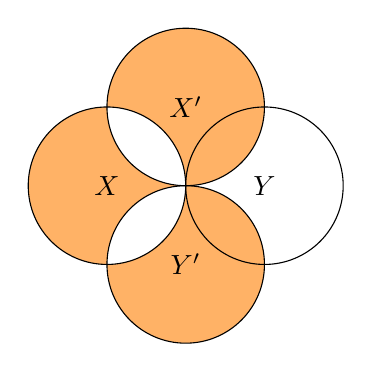
\begin{tikzpicture}
                \thiswithoutthose{\xset}{\xprimeset \yprimeset}
                \thiswithoutthose{\xprimeset}{\xset}
                \thiswithoutthose{\yprimeset}{\xset}
                \setboundaries
            \end{tikzpicture}
    }
    \quad
    \subfloat[$(X \cup Y) \symdiff X'$]{%
            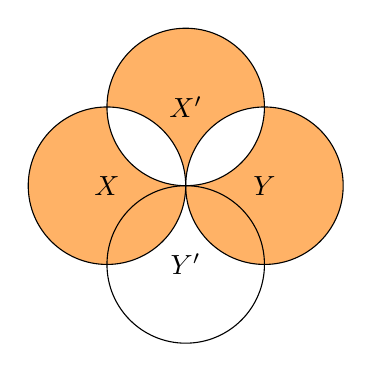
\begin{tikzpicture}
                \thiswithoutthose{\xset}{\xprimeset}
                \thiswithoutthose{\yset}{\xprimeset}
                \thiswithoutthose{\xprimeset}{\xset \yset}
                \setboundaries
            \end{tikzpicture}
    }
    \quad
    \subfloat[$X \symdiff X'$]{%
            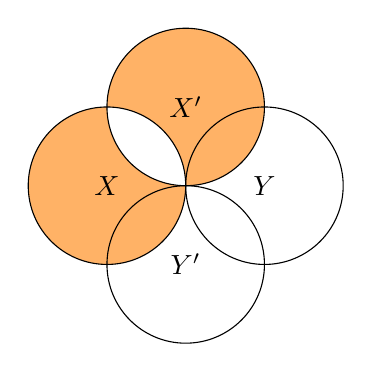
\begin{tikzpicture}
                \thiswithoutthose{\xset}{\xprimeset}
                \thiswithoutthose{\xprimeset}{\xset}
                \setboundaries
            \end{tikzpicture}
    }
    \quad
    \subfloat[$(X \cup Y) \symdiff (X' \cup Y')$]{%
            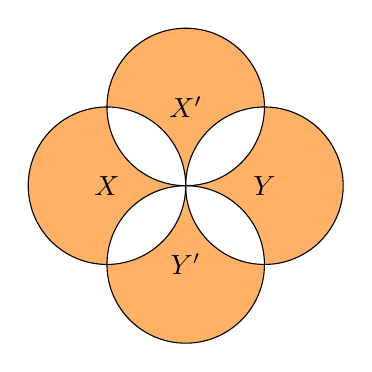
\begin{tikzpicture}
                \thiswithoutthose{\xset}{\xprimeset \yprimeset}
                \thiswithoutthose{\yset}{\xprimeset \yprimeset}
                \thiswithoutthose{\xprimeset}{\xset \yset}
                \thiswithoutthose{\yprimeset}{\xset \yset}
                \setboundaries
            \end{tikzpicture}
    }
    \caption{Depictions of the sets in \Cref{tourn_eqn_swap_lemma_symdiffs}}
    \label{tourn_fig_swap_lemma_venns}

\end{figure*}

\begin{proof}
    %
    Write $K'' = \swap{K'}{a_1}{a_2}$. It is clear that $K''$ has the chain
    property since $K'$ does. Since $K' \in \minch{K}$, we have $d(K, K'') \ge
    d(K, K')$. We will show that $d(K, K'') \le d(K, K')$ also, which implies
    $d(K, K'') = d(K, K') = \mindist{K}$ and thus $K'' \in \minch{K}$.

    To that end, observe that for any tournament $\hat{K}$,
    \[
        d(K, \hat{K}) = \sum_{a \in A}{|K(a) \symdiff \hat{K}(a)|}
    \]
    Noting that $K'(a) = K''(a)$ for $a \notin \{a_1,a_2\}$ and $K''(a_1) =
    K'(a_2)$, $K''(a_2) = K'(a_1)$, we have
    \begin{align*}
        d(K, K') - d(K, K'')
        &= \sum_{i \in \{1,2\}}{\left(
            |K(a_i) \symdiff K'(a_i)| - |K(a_i) \symdiff K''(a_i)|
        \right)} \\
        &= |K(a_1) \symdiff K'(a_1)| - |K(a_1) \symdiff K'(a_2)| \\
        &\quad + |K(a_2) \symdiff K'(a_2)| - |K(a_2) \symdiff K'(a_1)|
    \end{align*}

    To simplify notation, write $X = K(a_1)$, $X' = K'(a_2)$, $Y = K(a_2)
    \setminus K(a_1)$ and $Y' = K'(a_1) \setminus K'(a_2)$ so that
    \begin{align*}
        K(a_1) = X;
            &\quad\quad
        K(a_2) = X \cup Y \\
        K'(a_1) = X' \cup Y';
            &\quad\quad
        K'(a_2) = X'
    \end{align*}
    and $X \cap Y = X' \cap Y' = \emptyset$. Rewriting the above we have
    \begin{align*}
        d(K, K') - d(K, K'')
        &= |K(a_1) \symdiff K'(a_1)|
           + |K(a_2) \symdiff K'(a_2)|
            \\
        &  \quad
           - |K(a_1) \symdiff K'(a_2)|
           - |K(a_2) \symdiff K'(a_1)| \\
        &= |X \symdiff (X' \cup Y')|
           + |(X \cup Y) \symdiff X'| \\
        &  \quad
           -
           |X \symdiff X'|
           - |(X \cup Y) \symdiff (X' \cup Y')|
           % Number the final equation in the align* environment
           % Code courtesy of https://tex.stackexchange.com/a/42728
           \addtocounter{equation}{1}\tag{\theequation}
           \label{tourn_eqn_swap_lemma_symdiffs}
    \end{align*}

    Each of the symmetric differences in \cref{tourn_eqn_swap_lemma_symdiffs} are
    depicted in \Cref{tourn_fig_swap_lemma_venns}. Note that each of these sets can
    be expressed as a union of the 8 disjoint subsets of $X \cup Y \cup X' \cup
    Y'$ shown in the figure. Expanding the symmetric differences in
    \cref{tourn_eqn_swap_lemma_symdiffs} and consulting \Cref{tourn_fig_swap_lemma_venns},
    it can be seen that most terms cancel out, and in fact we are left with
    \[
        d(K, K') - d(K, K'') = 2|Y \cap Y'|  \ge 0
    \]
    This shows that $d(K, K'') \le d(K, K')$, and the proof is complete.
\end{proof}

\begin{notation}
    For a relation $R$ on a set $X$ and $x \in X$, write
    \[ U(x, R) = \{y \in X \mid x \mathrel{R} y\} \]
    \[ L(x, R) = \{y \in X \mid y \mathrel{R} x\} \]
    for the upper- and lower-sets of $x$ respectively.
\end{notation}

\begin{lemma}
    \label{tourn_result_chainmin_mon_extend_strict_part}
    For any tournament $K$ there is $K' \in \minch{K}$ such that for all $a \in
    A$:
    \[
        U(a, {\anlt_K}) \subseteq U(a, {\anle_{K'}})
    \]
    That is, $K(a) \subset K(a')$ implies $K'(a) \subseteq K'(a')$ for all $a,
    a' \in A$.
\end{lemma}

\begin{proof}
    %
    Write $A = \{a_1,\ldots,a_m\}$, ordered such that $|L(a_1, {\anle_K})| \le
    \cdots \le |L(a_m, {\anle_K})|$. We will show by induction that for each $0
    \le i \le m$ there is $K_i \in \minch{K}$ such that:
    \[
        1 \le j \le i
        \implies
        U(a_j, {\anlt_K}) \subseteq U(a_j, {\anle_{K_i}})
        \tag{$\ast$}
        \label{tourn_eqn_mon_lemma_induction}
    \]
    The result follows by taking $K' = K_m$.

    The case $i=0$ is vacuously true, and we may take $K_0$ to be an arbitrary
    member of $\minch{K}$. For the inductive step, suppose
    \labelcref{tourn_eqn_mon_lemma_induction} holds for some $0 \le i < m$. If
    $U(a_{i+1}, {\anlt_K}) = \emptyset$ then we may set $K_{i+1} = K_i$, so
    assume that $U(a_{i+1}, {\anlt_K})$ is non-empty. Take some $\hat{a} \in
    \min(U(a_{i+1}, {\anlt_K}), {\anle_{K_i}})$. Then $\hat{a}$ has (one of)
    the smallest neighbourhoods in $K_i$ amongst those in $A$ with a strictly
    larger neighbourhood than $a_{i+1}$ in $K$.

    If $K_i(a_{i+1}) \subseteq K_i(\hat{a})$ then we claim
    \labelcref{tourn_eqn_mon_lemma_induction} holds with $K_{i+1} = K_i$. Indeed, for
    $j < i + 1$ the inclusion in \labelcref{tourn_eqn_mon_lemma_induction} holds
    since it does for $K_i$. For $j = i+1$, let $a \in U(a_{i+1}, {\anlt_K})$.
    The definition of $\hat{a}$ implies $K_i(a) \not\subset K_i(\hat{a})$;
    since $K_i$ has the chain property this means $K_i(\hat{a}) \subseteq
    K_i(a)$. Consequently $K_i(a_{i+1}) \subseteq K_i(\hat{a}) \subseteq
    K_i(a)$, i.e. $a \in U(a_{i+1}, {\anle_{K_i}}) = U(a_{i+1},
    {\anle_{K_{i+1}}})$ as required.

    For the remainder of the proof we therefore suppose $K_i(a_{i+1})
    \not\subseteq K_i(\hat{a})$. The chain property for $K_i$ gives
    $K_i(\hat{a}) \subset K_i(a_{i+1})$. Since $K_i \in \minch{K}$ and
    $K(a_{i+1}) \subset K(\hat{a})$, we may apply
    \Cref{tourn_result_chainmin_mon_swapping}. Set $K_{i+1} =
    \swap{K_i}{a_{i+1}}{\hat{a}} \in \minch{K}$. The inclusion in
    \labelcref{tourn_eqn_mon_lemma_induction} is easy to show for $j=i+1$: if $a \in
    U(a_{i+1}, {\anlt_K})$ then either $a = \hat{a}$ -- in which case
    $K_{i+1}(a_{i+1}) \subset K_{i+1}(a)$ by construction -- or $a \ne \hat{a}$
    and $K_{i+1}(a_{i+1}) = K_i(\hat{a}) \subseteq K_i(a) = K_{i+1}(a)$. In
    either case $a \in U(a_{i+1}, {\anle_{K_{i+1}}})$ as required.

    Now suppose $1 \le j < i + 1$. First note that due to our assumption on the
    ordering of $\{a_1,\ldots,a_m\}$, we have $a_j \ne \hat{a}$ (indeed, if
    $a_j = \hat{a}$ then $K(a_{i+1}) \subset K(a_j)$ and $|L(a_j, {\anlt_K})| >
    |L(a_{i+1}, {\anlt_K})|$). Since $a_j \ne a_{i+1}$ also, $a_j$ was not
    involved in the swapping in the construction of $K_{i+1}$, and consequently
    $K_{i+1}(a_j) = K_i(a_j)$. Let $a \in U(a_j, {\anlt_K})$. We must show that
    $K_{i+1}(a_j) \subseteq K_{i+1}(a)$. We consider cases.

    \textbf{Case 1:} $a = \hat{a}$. Using the fact that
    \labelcref{tourn_eqn_mon_lemma_induction} holds for $K_i$ we have
    \[
        K_{i+1}(a_j)
        = K_i(a_j)
        \subseteq K_i(\hat{a})
        \subset K_i(a_{i+1})
        = K_{i+1}(\hat{a})
    \]

    \textbf{Case 2:} $a = a_{i+1}$. Here $K(a_j) \subset K(a_{i+1}) \subset
    K(\hat{a})$, i.e. $\hat{a} \in U(a_j, {\anlt_K})$. Applying the inductive
    hypothesis again we have
    \[
        K_{i+1}(a_j)
        = K_i(a_j)
        \subseteq K_i(\hat{a})
        = K_{i+1}(a_{i+1})
    \]

    \textbf{Case 3:} $a \notin \{\hat{a}, a_{i+1}\}$. Here neither $a_j$ nor
    $a$ were involved in the swap, so $K_{i+1}(a_j) = K_i(a_j) \subseteq K_i(a)
    = K_{i+1}(a)$.

    By induction, the proof is complete.
    %
\end{proof}

\begin{lemma}
    \label{tourn_result_chainmin_mon_extend_full}
    Let $K$ be a tournament and suppose $K' \in \minch{K}$ is such that $U(a,
    {\anlt_K}) \subseteq U(a, {\anle_{K'}})$ for all $a \in A$. Then there is
    $K'' \in \minch{K}$ such that ${\anle_K} \subseteq {\anle_{K''}}$.

    % $U(a, {\anle_K}) \subseteq U(a,
    % {\anle_{K''}})$.

\end{lemma}

\begin{proof}
    %
    Let $A_1, \ldots, A_t \subseteq A$ be the equivalence classes of
    ${\aneq_K}$, the symmetric part of ${\anle_K}$. Note that $a \aneq_K a'$
    iff $K(a) = K(a')$, so we can associate each $A_i$ with a neighbourhood
    $B_i \subseteq B$ such that $K(a) = B_i$ whenever $a \in A_i$.

    Our aim is to select a single element from each equivalence class $A_i$,
    which we denote by $f(A_i)$, and modify $K'$ to set the neighbourhood of
    each $a \in A_i$ to $K'(f(A_i))$. To that end, construct a function $f:
    \{A_1,\ldots,A_t\} \to A$ such that
    \[
        f(A_i) \in \argmin_{a \in A_i}{|B_i \symdiff K'(a)|} \in A_i
    \]
    Define $K''$ by $K''_{ab} = K'_{f([a]), b}$, where $[a]$ denotes the
    equivalence class of $a$. Then $K''(a) = K'(f([a]))$ for all $a$.

    Next we show that $K'' \in \minch{K}$. Note that $K''$ has the chain
    property, since $a_1 \anle_{K''} a_2$ iff $f([a_1]) \anle_{K'} f([a_2])$,
    and $f([a_1]), f([a_2])$ are guaranteed to be comparable with respect to
    ${\anle_{K'}}$ since $K'$ has the chain property. To show $d(K, K'')$ is
    minimal, observe that
    \begin{align*}
        d(K, K'')
        &= \sum_{a \in A}{|K(a) \symdiff K''(a)|} \\
        &= \sum_{i=1}^{t}{
            \sum_{a \in A_i}{
                |B_i \symdiff K'(f(A_i))|
            }
        }
    \end{align*}
    By definition of $f$, we have $|B_i \symdiff K'(f(A_i))| \le |B_i \symdiff
    K'(a)|$ for all $a \in A_i$. Consequently
    \begin{align*}
        d(K, K'')
        &\le \sum_{i=1}^{t}{
            \sum_{a \in A_i}{
                |B_i \symdiff K'(a)|
            }
        } \\
        &= d(K, K') \\
        &= \mindist{K}
    \end{align*}
    which implies $K'' \in \minch{K}$.

    We are now ready to prove the result. Suppose $a \anle_K a'$ i.e. $K(a)
    \subseteq K(a')$. If $K(a) = K(a')$ then $[a] = [a']$, so
    \[
        K''(a) = K'(f([a])) = K'(f([a'])) = K''(a')
    \]
    and in particular $K''(a) \subseteq K''(a')$. If instead $K(a) \subset
    K(a')$, then $K(f([a])) = K(a) \subset K(a') = K(f([a']))$, i.e.  $f([a])
    \anlt_K f([a'])$. By the assumption on $K'$ in the statement of the lemma,
    this means $f([a]) \anle_{K'} f([a'])$, and so
    \[
        K''(a) = K'(f([a])) \subseteq K'(f([a'])) = K''(a')
    \]
    In either case $K''(a) \subseteq K''(a')$, i.e. $a \anle_{K''} a'$. Since
    $a, a'$ were arbitrary, this shows that ${\anle_K} \subseteq {\anle_{K''}}$
    as required.
    %
\end{proof}

The pieces are now in place to prove \Cref{tourn_result_chainmin_mon_compatibility}

\begin{proof}[Proof of \Cref{tourn_result_chainmin_mon_compatibility}]
    %
    For any tournament $K$, write
    \[
        \minchmon{K} = \{
            K' \in \minch{K} \mid {\anle_K} \subseteq {\anle_{K'}}
        \}
    \]
    By \Cref{tourn_result_chainmin_mon_extend_strict_part} and
    \Cref{tourn_result_chainmin_mon_extend_full}, $\minchmon{K}$ is non-empty. Let
    $\ll$ be any total order on the set $\K$ of all tournaments.
    Define a function $\alpha: \K \to \K$ by
    \[
        \alpha(K) = \min(\minchmon{K}, {\ll}) \in \minchmon{K}
    \]
    Note that the minimum is unique since ${\ll}$ is a total order. Defining an
    operator $\phi$ by $\phi(K) = ({\anle_{\alpha(K)}}, {\bnle_{\alpha(K)}})$,
    we see that $\phi$ satisfies \axiomref{chain-min} and \axiomref{mon}, as
    required.
    %
\end{proof}

\section{Proof of \Cref{tourn_prop_matchpref_weightings}}

The following preliminary result is required.

\begin{lemma}
   \label{tourn_result_powertwo}

   Let $k$ and $l$ be integers with $1 \le k \le l$. Then
   \[ \sum_{i=k}^{l}{2^{-i}} < 2^{-(k - 1)} \]

\end{lemma}

\begin{proof}

    This follows from the formula for the sum of a finite geometric
    series:
    %\footnote{\url{https://en.wikipedia.org/wiki/Geometric\_series\#Formula}}
    \[
        \sum_{i=0}^{n-1}{r^i} = \frac{1-r^n}{1-r}
    \]
    which holds for all $r \ne 1$. In this case we have
    \begin{align*}
        \sum_{i=k}^{l}{2^{-i}}
        &= \sum_{i=0}^{l}{2^{-i}} - \sum_{i=0}^{k-1}{2^{-i}} \\
        &= \sum_{i=0}^{l}{\left(\frac{1}{2}\right)^i}
           -
           \sum_{i=0}^{k - 1}{\left(\frac{1}{2}\right)^i} \\
        &= \frac{
               1 - \left(\frac{1}{2}\right)^{l+1}
           }{
               1 - \left(\frac{1}{2}\right)
           }
           -
           \frac{
               1 - \left(\frac{1}{2}\right)^k
           }{
               1 - \left(\frac{1}{2}\right)
           } \\
        &= 2 \left(
           2^{-k} - 2^{-(l+1)}
        \right) \\
        &= 2^{-(k-1)} - \underbrace{2^{-l}}_{> 0} \\
        &< 2^{-(k-1)}
    \end{align*}
    as required.
\end{proof}

\begin{proof}[Proof of \Cref{tourn_prop_matchpref_weightings}]

    Let $\trianglelefteq$ be a total order on $\N \times \N$ and let $m, n \in
    \N$. For $a \in [m]$ and $b \in [n]$, write
    \[
        p(a,b)
        =
        1 + |\{(a',b') \in [m] \times [n] : (a',b') \vartriangleleft (a,b)\}|
    \]
    for the `position' of $(a,b)$ in ${\trianglelefteq} \rs ([m] \times [n])$
    (where 1 corresponds to the minimal pair). Define $w$ by
    \[
        w(a,b) = 1 + 2^{-p(a,b)}
    \]
    If we abuse notation slightly and view $w$ as an $m \times n$ matrix, we
    have, by construction, $\vect_{\trianglelefteq}(w) = (1 +
    2^{-1},\ldots,1 + 2^{-mn})$. Noting that $|K_{ab} - K'_{ab}| = [K \oplus
    K']_{ab}$ for any tournaments $K, K'$, and letting $\dotprod$ denote the
    dot product, it is easy to see that
    \begin{align*}
        d_w(K, K')
        &= \vect_{\trianglelefteq}(w)
            \dotprod \vect_{\trianglelefteq}(K \oplus K') \\
        &= (1 + 2^{-1},\ldots,1 + 2^{-mn})
           \dotprod
           \vect_{\trianglelefteq}(K \oplus K') \\
        &= d(K, K') + \bm{x} \dotprod \vect_{\trianglelefteq}(K \oplus K')
    \end{align*}
    where $\bm{x} = (2^{-1},\ldots,2^{-mn})$ and $d(K, K')$ is the
    unweighted Hamming distance. In particular, since $\bm{x}$ and
    $\vect_{\trianglelefteq}(K \oplus K')$ are non-negative, we have $d_w(K, K')
    \ge d(K, K')$.

    Now, we will show that for any $m \times n$ tournament $K$ and $K' \in
    \ch_{m,n}$ with $K' \ne \alpha_{\trianglelefteq}(K)$ we have $d_w(K,
    \alpha_{\trianglelefteq}(K)) < d_w(K, K')$. Since
    $\alpha_{\trianglelefteq}(K) \in \minch{K} \subseteq \ch_{m,n}$ by
    definition, this will show that $\alpha_{\trianglelefteq}(K)$ is the
    unique minimum in \Cref{tourn_eqn_matchpref_argmin}, as required.

    So, let $K$ be an $m \times n$ tournament and $K' \in \ch_{m,n}$. To ease
    notation, write $v = \vect_{\trianglelefteq}(K \oplus
    \alpha_{\trianglelefteq}(K))$ and $v' = \vect_{\trianglelefteq}(K \oplus K')$.
    There are two cases.

    \textbf{Case 1:} $K' \not\in \minch{K}$. In this case we have $d(K, K')
    \ge \mindist{K} + 1$, and
    \begin{align*}
       d_w(K, \alpha_{\trianglelefteq}(K))
       &=
           \underbrace{d(K, \alpha_{\trianglelefteq}(K))}_{= \mindist{K}}
           +
           \bm{x} \dotprod v \\
       &= \mindist{K} + \sum_{i=1}^{mn}{2^{-i} \cdot \underbrace{v_i}_{\le 1}}
       \\
       &\le \mindist{K} + \underbrace{\sum_{i=1}^{mn}{2^{-i}}}_{< 2^{-0} = 1}
       \\
       &< \mindist{K} + 1 \\
       &\le d(K, K') \\
       &\le d_w(K, K')
    \end{align*}
    where \Cref{tourn_result_powertwo} was applied in the 4th step. This shows $d_w(K,
    \alpha_{\trianglelefteq}(K)) < d_w(K, K')$, as required.

    \textbf{Case 2:} $K \in \minch{K}$. In this case we have
    \begin{align*}
       d(K, \alpha_{\trianglelefteq}(K)) - d(K, K')
       &= (\mindist{K} + \bm{x} \dotprod v)
          -
          (\mindist{K} + \bm{x} \dotprod v') \\
       &= \bm{x} \dotprod (v - v')
    \end{align*}

    Now, since $K' \in \minch{K}$, $v'$ appears as one of the vectors over
    which the $\argmin$ is taken in
    \Cref{tourn_eqn_match_preference_alpha_definition}. By definition of
    $\alpha_{\trianglelefteq}$ we therefore know that $v$ strictly precedes
    $v'$ with respect to the lexicographic order on $\{0,1\}^{mn}$.
    Consequently there is $j \ge 1$ such that $v_i = v'_i$ for $i < j$ and $v_j
    < v'_j$. That is, $v_j = 0$ and $v'_j = 1$. This means
    %
    \begin{align*}
       d(K, \alpha_{\trianglelefteq}(K)) - d(K, K')
       &= \bm{x} \dotprod (v - v') \\
       &= \sum_{i=1}^{mn}{2^{-i}(v_i - v'_i)} \\
       &= \sum_{i=1}^{j-1}{2^{-i}\underbrace{(v_i - v'_i)}_{=0}}
          +
          \sum_{i=j}^{mn}{2^{-i}(v_i - v'_i)} \\
       &= 2^{-j}\underbrace{(v_j - v'_j)}_{=-1}
          + \sum_{i=j + 1}^{mn}{
               2^{-i}
               \underbrace{(v_i - v'_i)}_{\le 1}
            } \\
       &\le -2^{-j}
            + \sum_{i=j+1}^{mn}{
                  2^{-i}
              } \\
       &< -2^{-j} + 2^{-j} \\
       &= 0
    \end{align*}
    where \Cref{tourn_result_powertwo} was applied in the second to last step.
    Again, this shows $d_w(K, \alpha_{\trianglelefteq}(K)) < d_w(K, K')$, and
    the proof is complete.
\end{proof}

\section{Proof of \Cref{tourn_result_chain_def_ranks_characterisation}}

\begin{proof}

    First we set up some notation. For a total preorder $\preceq$ on a set $Z$
    and $z \in Z$, write $[z]_{\preceq}$ for the rank of ${\preceq}$ containing
    $z$, i.e. the equivalence class of $z$ in the symmetric closure of
    ${\preceq}$:
    \[
        [z]_{\preceq}
        = \{z' \in Z \mid z \preceq z' \text{ and } z' \preceq z\}
    \]
    Also note that $\preceq$ can be extended to a total order on the ranks by
    setting $[z]_{\preceq} \le [z']_{\preceq}$ iff $z \preceq z'$.

    (⇒) We start with the `only if' statement of the theorem. Suppose
    $\phi$ satisfies \axiomref{chain-def}, and let $K$ be a tournament. We need
    to show that $|\ranks{\ale_K^\phi} - \ranks{\ble_K^\phi}| \le 1$.

    By chain-definability, there is $K'$ with the chain property such that $a
    \ale_K^\phi a'$ iff $K'(a) \subseteq K'(a')$ and $b \ble_K^\phi b'$ iff
    $(K')^{-1}(b) \supseteq (K')^{-1}(b')$. Write
    \[ \mathcal{X} = \{ [a]_{\ale_K^\phi} \mid a \in A, K'(a) \ne \emptyset \} \]
    \[ \mathcal{Y} = \{ [b]_{\ble_K^\phi} \mid b \in B, (K')^{-1}(b) \ne \emptyset \} \]
    for the set of ranks in each of the two orders, excluding those who have
    empty neighbourhoods in $K'$. Note that $[a]_{\ale_K^\phi} =
    [a']_{\ale_K^\phi}$ if and only if $K'(a) = K'(a')$ (and similar for $B$).

    We will show that $|\mathcal{X}| = |\mathcal{Y}|$. Enumerate $\mathcal{X} =
    \{X_1,\ldots,X_s\}$ and $\mathcal{Y} = \{Y_1,\ldots,Y_t\}$, ordered such
    that $X_1 < \cdots < X_s$ and $Y_1 < \cdots < Y_t$. First we show
    $|\mathcal{X}| \le |\mathcal{Y}|$.

    For each $1 \le i \le s$, the $a_i$ be an arbitrary element of $X_i$. Then
    $a_1 \alt_K^\phi \cdots \alt_K^\phi a_s$, so $\emptyset \subset K'(a_1)
    \subset \cdots \subset K'(a_s)$. Since these inclusions are strict, we can
    choose $b_1,\ldots,b_s \in B$ such that $b_1 \in K'(a_1)$ and $b_{i+1} \in
    K'(a_{i+1}) \setminus K'(a_i)$ for $1 \le i < s$.

    It follows that $a_i \in (K')^{-1}(b_i) \setminus (K')^{-1}(b_{i+1})$, and
    thus $(K')^{-1}(b_i) \not\subseteq (K')^{-1}(b_{i+1})$. Since $K'$ has
    the chain property, this means $(K')^{-1}(b_{i+1}) \subset
    (K')^{-1}(b_i)$, i.e. $b_i \blt_K^\phi b_{i+1}$.

    We now have $b_1 \blt_K^\phi \cdots \blt_K^\phi b_s$; a chain of $s$ strict
    inequalities in $\ble_K^\phi$. The corresponding ranks $[b_1], \ldots,
    [b_s]$ are all distinct and lie inside $\mathcal{Y}$. But now we have found
    $s = |\mathcal{X}|$ distinct elements of $\mathcal{Y}$, so $|\mathcal{X}|
    \le |\mathcal{Y}|$ as promised.

    Repeating this argument with the roles of $\mathcal{X}$ and $\mathcal{Y}$
    interchanged, we find that $|\mathcal{Y}| \le |\mathcal{X}|$ also, and
    therefore $|\mathcal{X}| = |\mathcal{Y}|$.

    To conclude, note that $\ranks{\ale_K^\phi} \in \{|\mathcal{X}|,
    |\mathcal{X}| + 1\}$, since there can exist at most one rank which was
    excluded from $\mathcal{X}$ (namely, those $a \in A$ with $K'(a) =
    \emptyset$). For identical reasons, $\ranks{\ble_K^\phi} \in
    \{|\mathcal{Y}|, |\mathcal{Y}| + 1\}$. Since $|\mathcal{X}| =
    |\mathcal{Y}|$, it is clear that $\ranks{\ale_K^\phi}$ and
    $\ranks{\ble_K^\phi}$ can differ by at most one, as required.

    (⇐) Now we prove the `if' statement. Let $K$ be a tournament. We have
    $|\ranks{\ale_K^\phi} - \ranks{\ble_K^\phi}| \le 1$, and must show there is
    tournament $K'$ with the chain property such that $\phi(K) = ({\anle_{K'}},
    {\bnle_{K'}})$.

    Let $X_1 < \cdots < X_s$ and $Y_1 < \cdots < Y_t$ be the ranks of
    $\ale_K^\phi$ and $\ble_K^\phi$ respectively. By hypothesis $|s - t| \le
    1$. Define $g: \{1,\ldots,s\} \to \{0,\ldots,t\}$ by
    \[
        g(i) = \begin{cases}
            i,& s \in \{t-1, t\} \\
            i - 1,& s = t + 1
        \end{cases}
    \]
    Not that the two cases above cover all possibilities, since $|s - t| \le
    1$. For $i \in [s]$, write
    \[
        N_i = \bigcup_{0 \le j \le g(i)}{Y_j}
    \]
    where $Y_0 := \emptyset$. Note that $g(i+1) = g(i) + 1$, and consequently
    \[
        N_{i+1}
        = \bigcup_{j \le g(i) + 1}{Y_j}
        = N_i \cup Y_{g(i) + 1}
        = N_i \cup Y_{g(i + 1)}
    \]
    Since $g(i+1) > 0$ we have $Y_{g(i+1)} \ne \emptyset$, and thus $N_{i+1}
    \supset N_i$ for all $i < s$.

    Now, for any $a \in A$, let $p(a) \in [s]$ be the unique integer such that
    $a \in X_{p(a)}$; such $p(a)$ always exists since $\{X_1,\ldots,X_s\}$ is a
    partition of $A$. Note that due to the assumption on the ordering of the
    $X_i$, we have $a \ale_K^\phi a'$ if and only if $p(a) \le p(a')$.

    Let $K'$ be the unique tournament such that $K'(a) = N_{p(a)}$ for each $a
    \in A$. Since $N_1 \subset \cdots \subset N_p$, we have
    \begin{equation}
        \label{tourn_eqn_ale_k_phi_iff_anle_kprime}
        \begin{aligned}
            a \ale_K^\phi a'
            &\iff p(a) \le p(a') \\
            &\iff N_{p(a)} \subseteq N_{p(a')} \\
            &\iff K'(a) \subseteq K'(a') \\
            &\iff a \anle_{K'} a'
        \end{aligned}
    \end{equation}
    i.e. ${\ale_K^\phi} = {\anle_{K'}}$. Since ${\ale_K^\phi}$ is a total
    preorder, this shows that $K'$ has the chain property.

    It only remains to show that ${\ble_K^\phi} = {\bnle_{K'}}$. First note
    that if $a \in X_i$ and $b \in Y_j$, the fact that $\{Y_1,\ldots,Y_t\}$ are
    disjoint implies
    \begin{align*}
        a \in (K')^{-1}(b)
        &\iff b \in K'(a) = N_i = \bigcup_{0 \le k \le g(i)}{Y_k} \\
        &\iff j \le g(i)
    \end{align*}
    Hence $(K')^{-1}(b)$ only depends on $j$: every $b \in Y_j$ shares the same
    neighbourhood $M_j$, given by
    \[
        M_j = \bigcup_{i \in [s] :\ g(i) \ge j}{X_i}
    \]
    Note that if $1 \le j < t$,
    \begin{align*}
        M_j
        &= \bigcup_{i \in [s] :\ g(i) \ge j}{X_i} \\
        &= \left(\bigcup_{i \in [s] :\ g(i) \ge j + 1}{X_i}\right)
            \cup
            \left(\bigcup_{i \in g^{-1}(j)}{X_i}\right) \\
        &= M_{j+1} \cup \bigcup_{i \in g^{-1}(j)}{X_i}
    \end{align*}
    Since $1 \le j < t$ we have
    \[
        g^{-1}(j) = \begin{cases}
            \{j\},& s \in \{t-1,t\} \\
            \{j+1\},& s = t + 1
        \end{cases}
    \]
    In particular $g^{-1}(j) \ne \emptyset$, which means $\bigcup_{i \in
    g^{-1}(j)}{X_i} \ne \emptyset$ and thus $M_j \supset M_{j+1}$
    for all $1 \le j < t$.

    Finally, since $(K')^{-1}(b) = M_j$ for $b \in Y_j$ and $M_1 \supset \cdots
    \supset M_t$, an argument almost identical to
    \labelcref{tourn_eqn_ale_k_phi_iff_anle_kprime} shows that ${\ble_K^\phi} =
    {\bnle_{K'}}$.

    We have shown that $\phi(K) = ({\anle_{K'}}, {\bnle_{K'}})$ and that $K'$
    has the chain property, and the proof is therefore complete.
\end{proof}

\section{Proof that the interleaving procedure eventually terminates}

\begin{proposition}
    \label{tourn_prop_interleaving_terminates}

    Let $(f,g)$ be selection functions. Fix a tournament $K$ and let $A_i,
    B_i$ ($i \ge 0$) be as in \Cref{tourn_def_interleaving}. Then there are $j, j'
    \ge 1$ such that $A_j = \emptyset$ and $B_{j'} = \emptyset$. Moreover,
    there is $t \ge 1$ such that both $A_t = B_t = \emptyset$.

\end{proposition}

\begin{proof}

    Suppose $i \ge 0$ and $A_i \ne \emptyset$. Then properties
    \labelcref{tourn_item_f_sel_1} and \labelcref{tourn_item_f_sel_2} for $f$ in
    \Cref{tourn_def_selectionfunction} imply that $\emptyset \subset f(K, A_i, B_i)
    \subseteq A_i$, and consequently $A_{i+1} = A_i \setminus f(K, A_i, B_i)
    \subset A_i$.

    Supposing that $A_j \ne \emptyset$ for all $j \ge 0$, we would have $A_0
    \supset A_1 \supset A_2 \supset \cdots$ which clearly cannot be the case
    since each $A_j$ lies inside $A$ which is a finite set. Hence there is $j
    \ge 1$ such that $A_j = \emptyset$. Moreover, since $A_j \supseteq A_{j+1}
    \supseteq A_{j+2} \supseteq \cdots$, we have $A_k = \emptyset$ for all $k
    \ge j$.

    An identical argument with $g$ shows that there is $j' \ge 1$ such that
    $B_{j'} = \emptyset$ and $B_k = \emptyset$ for all $k \ge j'$.

    Taking $t = \max\{j, j'\}$, we have $A_t = B_t = \emptyset$ as required.
\end{proof}

\section{Proof of \Cref{tourn_result_chaindef_iff_interleaving}}

\begin{proof}

    Throughout the proof we will refer to a pair of total preorders
    $({\ale}, {\ble})$ as `chain-definable' if there is a chain tournament $K$
    such that ${\ale} = {\anle_K}$ and ${\ble} = {\bnle_K}$.

    (⇐) First we prove the `if' direction. Let $\phi = \intop{f,g}$ be an
    interleaving operator with selection functions $(f, g)$, and fix a
    tournament $K$. We will show that $\phi(K)$ is chain-definable.

    As per \Cref{tourn_prop_interleaving_terminates}, let $j, j' \ge 1$ be the
    minimal integers such that $A_j = \emptyset$ and $B_{j'} = \emptyset$. Then
    we have $A_0 \supset \cdots \supset A_{j-1} \supset A_j = \emptyset$ and
    $B_0 \supset \cdots \supset B_{j'-1} \supset B_{j'} = \emptyset$.

    Recall that, for $a \in A$, we have by definition $r(a) = \max\{i \mid a
    \in A_i\}$, which is the unique integer such that $a \in A_{r(a)} \setminus
    A_{{r(a)}+1}$. Since $a \ale_K^\phi a'$ iff $r(a) \ge r(a')$, it follows
    that the non-empty sets $A_0 \setminus A_1, \ldots, A_{j-1} \setminus A_j$
    form the ranks of the total preorder ${\ale_K^\phi}$ (that is, the
    equivalence classes of the symmetric closure ${\aeq_K^\phi}$). Thus,
    ${\ale_K^\phi}$ has $j$ ranks. An identical argument shows that
    ${\ble_K^\phi}$ has $j'$ ranks.

    It follows from \Cref{tourn_result_chain_def_ranks_characterisation} that $\phi(K)$
    is chain-definable if and only if $|j - j'| \le 1$.  If $j = j'$ this is
    clear. Suppose $j < j'$.  Then $A_j = \emptyset$ and $B_j \ne \emptyset$.
    By property \labelcref{tourn_item_g_sel_3} for $g$ in
    \Cref{tourn_def_selectionfunction}, we have $g(K, A_j, B_j) = g(K, \emptyset,
    B_j) = B_j$. But this means $B_{j+1} = B_j \setminus g(K, A_j, B_j) = B_j
    \setminus B_j = \emptyset$.  Consequently $j' = j+1$, and $|j - j'| = |-1|
    = 1$

    If instead $j > j'$, then a similar argument using property
    \labelcref{tourn_item_f_sel_3} for $f$ in \Cref{tourn_def_selectionfunction} shows
    that $j = j' + 1$, and we have $|j - j'| = |1| = 1$.

    Hence $|j - j'| \le 1$ in all cases, and $\phi(K)$ is chain-definable as
    required.

    (⇒) Now for the `only if' direction. Suppose $\phi$ satisfies
    \axiomref{chain-def}. We will define $f, g$ such that $\phi = \intop{f,g}$.
    The idea behind the construction is straightforward: since $f$ and $g$ pick
    off the next-top-ranked $A$s and $B$s at each iteration, simply define
    $f(K, A_i, B_i)$ as the maximal elements of $A_i$ with respect to the
    existing ordering ${\ale_K^\phi}$ ($g$ will be defined similarly). The
    interleaving algorithm will then select the ranks of ${\ale_K^\phi}$ and
    ${\ble_K^\phi}$ one-by-one; the fact that $\phi(K)$ is chain-definable
    ensures that we select \emph{all} the ranks before the iterative procedure
    ends. The formal details follow.

    Fix a tournament $K$. By \Cref{tourn_result_chain_def_ranks_characterisation},
    $|\ranks{{\ale_K^\phi}} - \ranks{{\ble_K^\phi}}| \le 1$. Taking $t =
    \max\{\ranks{{\ale_K^\phi}}, \ranks{{\ble_K^\phi}}\}$, we can write $X_1,
    \ldots, X_t \subseteq A$ and $Y_1, \ldots, Y_t \subseteq B$ for the ranks
    of ${\ale_K^\phi}$ and ${\ble_K^\phi}$ respectively, possibly with $X_1 =
    \emptyset$ if $\ranks{{\ble_K^\phi}} = 1 + \ranks{{\ale_K^\phi}}$ or $Y_1 =
    \emptyset$ if $\ranks{{\ale_K^\phi}} = 1 + \ranks{{\ble_K^\phi}}$. Note
    that $X_i, Y_i \ne \emptyset$ for $i > 1$. Assume these sets are ordered
    such that $a \ale_K^\phi a'$ iff $i \le j$ whenever $a \in X_i$ and $a' \in
    X_j$ (and similar for the $Y_i$). Also note that the $X_i \cap X_j =
    \emptyset$ for $i \ne j$ (and similar for the $Y_i$).

    Now set \footnotemark{}
    \[
        f(K, A', B') = \begin{cases}
           \max(A', {\ale_K^\phi}),& B' \ne \emptyset \\
           A',& B' = \emptyset
        \end{cases}
    \]
    \[
        g(K, A', B') = \begin{cases}
            \max(B', {\ble_K^\phi}),& A' \ne \emptyset \\
            B',& A' = \emptyset
        \end{cases}
    \]

    \footnotetext{
        Here $\max(Z, {\preceq}) = \{z \in Z \mid \not\exists z' \in Z : z
        \prec z'\}$, for any set $Z$ and a total preorder ${\preceq}$ on $Z$
        (with strict part ${\prec}$).
    }

    It is not difficult to see that $f$ and $g$ satisfy the conditions of
    \Cref{tourn_def_selectionfunction} for selection functions. We claim that for
    with $A_i, B_i$ denoting the interleaving sets for $K$ and $(f, g)$, for
    all $0 \le i \le t$ we have
    \begin{equation}
        \label{tourn_eqn_ai_bi_unions}
        A_i = \bigcup_{j=1}^{t - i}{X_j},
        \quad
        B_i = \bigcup_{j=1}^{t - i}{Y_j}
        \quad
        \quad
    \end{equation}
    For $i = 0$ this is clear: since $X_1,\ldots,X_t$ contains all ranks of
    ${\ale_K^\phi}$ we have $\bigcup_{j=1}^{t-0} = X_1 \cup \cdots \cup X_t = A
    = A_0$ (and similar for $B$).

    Now suppose \labelcref{tourn_eqn_ai_bi_unions} holds for some $0 \le i < t$. We
    will show that $f(K, A_i, B_i) = X_{t-i}$ by considering three possible
    cases, at least one of which must hold.

    \textbf{Case 1:} ($A_i \ne \emptyset$, $B_i \ne \emptyset$). Here we have
    \begin{align*}
        f(K, A_i, B_i)
        &= \max(A_i, {\ale_K^\phi}) \\
        &= \max(X_1 \cup \cdots \cup X_{t-i}, {\ale_K^\phi}) \\
        &= X_{t-i}
    \end{align*}
    since the $X_j$ form (disjoint) ranks of ${\ale_K^\phi}$ with $X_{j} \alt
    X_{k}$ for $j < k$.

    \textbf{Case 2:} ($B_i = \emptyset$). Here we have
    $\bigcup_{j=1}^{t-i}{Y_j} = \emptyset$. Since $t - i \ge 1$ and $Y_j \ne
    \emptyset$ for $j > 1$, it must be the case that $t - i = 1$ and $B_i = Y_1
    = \emptyset$. Consequently by the induction hypothesis we have $A_i =
    \bigcup_{j=1}^{1}{X_j} = X_1$, and thus
    \begin{align*}
        f(K, A_i, B_i)
        &= f(K, A_i, \emptyset) \\
        &= A_i \\
        &= X_1 \\
        &= X_{t-i}
    \end{align*}

    \textbf{Case 3:} ($A_i = \emptyset$). By a similar argument as in case 2,
    we must have $t - i = 1$ and $A_i = X_1 = \emptyset$. Using the fact that
    $f(K, A_i, B_i) \subseteq A_i$ we get
    \begin{align*}
        f(K, A_i, B_i)
        &= \underbrace{f(K, \emptyset, B_i)}_{\subseteq \emptyset} \\
        &= \emptyset \\
        &= X_1 \\
        &= X_{t-i}
    \end{align*}
    We have now covered all cases, and have shown that $f(K, A_i, B_i) =
    X_{t-i}$ must hold. Consequently, using again the fact that the $X_j$ are
    disjoint,
    \begin{align*}
        A_{i+1}
        &= A_i \setminus f(K, A_i, B_i) \\
        &= \left(\bigcup_{j=1}^{t-i}{X_j}\right) \setminus X_{t-i} \\
        &= \bigcup_{j=1}^{t-(i+1)}{X_j}
    \end{align*}
    as required. By almost identical arguments we can show that $g(K, A_i, B_i)
    = Y_{t-i}$, and thus $B_{i+1} = \bigcup_{j=1}^{t-(i+1)}{Y_j}$ also. By
    induction, \labelcref{tourn_eqn_ai_bi_unions} holds for all $0 \le i \le t$.

    It remains to show that $a \ale_K^\phi a'$ iff $a \ale_K^{\intop{f,g}} a'$
    and that $b \ble_K^\phi b'$ iff $b \ble_K^{\intop{f,g}} b'$.

    For $a \in A$, let $p(a)$ be the unique integer such that $a \in X_{p(a)}$,
    i.e. $p(a)$ is the index of the rank of $a$ in the ordering
    ${\ale_K^\phi}$. Note that we have
    \[
        a \in A_i = X_1 \cup \cdots \cup X_{t-i}
        \iff
        t - i \ge p(a)
    \]
    and therefore
    \[
        r(a)
        = \max\{i \mid a \in A_i\}
        = \max\{i \mid t - i \ge p(a)\}
        = t - p(a)
    \]
    Using the fact that $X_i \alt X_j$ for $i < j$, we get
    \begin{align*}
        a \ale_K^{\intop{f,g}} a'
        &\iff r(a) \ge r(a') \\
        &\iff t - p(a) \ge t - p(a') \\
        &\iff p(a) \le p(a') \\
        &\iff a \ale_K^\phi a'
    \end{align*}
    A similar argument shows that $b \ble_K^\phi b'$ iff $b
    \ble_K^{\intop{f,g}} b'$ for any $b, b' \in B$. Since $K$ was arbitrary, we
    have shown that $\phi = \intop{f,g}$ as required.
\end{proof}

\section{Proof of \Cref{tourn_result_chaindef_axiom_compatibilities}}

\begin{proof}

    Since \axiomref{chain-min} implies \axiomref{chain-def},
    \Cref{tourn_result_chainmin_axiom_compatibilities} implies the existence of an
    operator with \axiomref{chain-def} and \axiomref{dual}, and an operator
    with \axiomref{chain-def} and \axiomref{mon}.  Moreover, the trivial
    operator which ranks all $A$s and $B$s equally satisfies \axiomref{anon}
    and \axiomref{IIM}. It only remains to show that there is an operator
    satisfying both \axiomref{chain-def} and \axiomref{pos-resp}.

    To that end, for any tournament $K$, define $K'$ by
    \[
        K'_{ab} = \begin{cases}
            1 ,& b \le |K(a)| \\
            0 ,& b > |K(a)|
        \end{cases}
    \]
    Note that $K'(a) = \{1,\ldots,|K(a)|\}$ for $|K(a)| > 0$. Consequently
    $K'(a) \subseteq K'(a')$ iff $|K(a)| \le |K(a)|$. We see that $K'$ has the
    chain property, and the operator $\phi$ defined by $\phi(K) =
    ({\anle_{K'}}, {\bnle_{K'}})$ satisfies \axiomref{chain-def}. In
    particular, $a \ale_K^\phi a'$ iff $|K(a)| \le |K(a')|$.

    To show \axiomref{pos-resp}, suppose $a \ale_K^\phi a'$ and $K_{a',b} = 0$
    for some $a, a' \in A$ and $b \in B$. Write $\hat{K} = K + \bm{1}_{a',b}$.

    Since $a \ale_K^\phi a'$ implies $|K(a)| \le |K(a')|$, we have
    $|\hat{K}(a')| = 1 + |K(a')| > |K(a)| = |\hat{K}(a)|$, and therefore $a
    \alt_{\hat{K}}^\phi a'$ as required for \axiomref{pos-resp}.
\end{proof}

\section{Proof of \Cref{tourn_result_chaindef_impossibility}}

\begin{proof}

    For contradiction, suppose there is an operator $\phi$ satisfying the
    stated axioms. Consider
    \[
        K = \left[\begin{smallmatrix}
            0 & 0 \\
            0 & 1 \\
            1 & 0 \\
            1 & 1
        \end{smallmatrix}\right]
    \]
    and two tournaments obtained by removing a single 1 entry:
    \[
        K_1 = \left[\begin{smallmatrix}
            0 & 0 \\
            0 & \bm{{\color{red}0}} \\
            1 & 0 \\
            1 & 1
        \end{smallmatrix}\right],
        \quad
        K_2 = \left[\begin{smallmatrix}
            0 & 0 \\
            0 & 1 \\
            1 & 0 \\
            1 & \bm{{\color{red}0}}
        \end{smallmatrix}\right]
    \]
    Now, \axiomref{anon} in $K_1$ gives $1 \aeq_{K_1}^\phi 2$ (e.g. take
    $\sigma = (1\ 2)$, $\pi = \text{id}_B$). In particular, $1 \ale_{K_1}^\phi
    2$, so \axiomref{pos-resp} implies $1 \alt_K^\phi 2$. A similar argument
    with $K_2$ shows that $3 \aeq_{K_2}^\phi 4$ and $3 \alt_K^\phi 4$.

    On the other hand, applying \axiomref{anon} to $K$ directly with $\sigma =
    (2\ 3)$ and $\pi = (1\ 2)$, we see that $2 \aeq_K^\phi 3$. The ranking of
    $A$ is thus fully determined as $1 \alt 2 \aeq 3 \alt 4$. In particular,
    $\ranks{\ale_K^\phi} = 3$.

    But now considering the dual tournament $\dual{K} =
    \left[\begin{smallmatrix} 1&1&0&0 \\ 1&0&1&0 \end{smallmatrix}\right]$ and
    applying permutations $\sigma = (1\ 2)$ and $\pi = (2\ 3)$, we obtain $1
    \aeq_{\dual{K}}^\phi 2$ by \axiomref{anon}, i.e. the $A$ ranking in
    $\dual{K}$ is flat. By \axiomref{dual} this implies the $B$ ranking in $K$
    is flat, i.e. $\ranks{\ble_K^\phi} = 1$. We see that $\ranks{\ale_K^\phi}$
    and $\ranks{\ble_K^\phi}$ differ by 2, contradicting \axiomref{chain-def}
    according to \Cref{tourn_result_chain_def_ranks_characterisation}.
\end{proof}

\section{Proof of \Cref{tourn_result_phicardint_axioms}}

We require a preliminary result providing sufficient conditions for an
interleaving operator $\intop{f,g}$ to satisfy various axioms.

\begin{lemma}
   \label{tourn_result_interleaving_suffconditions}

   Let $\phi = \phi_{f,g}^{\text{int}}$ be an interleaving operator.

   \begin{enumerate}
       \item \label{tourn_item_int_lemma_anon}

        If for any tournament $K$, $A' \subseteq A$, $B' \subseteq B$ and for
        any pair of permutations $\sigma: A \to A$ and $\pi: B \to B$ we have
        \begin{align*}
            f(\pi(\sigma(K)), \sigma(A'), \pi(B')) &= \sigma(f(K, A', B')) \\
            g(\pi(\sigma(K)), \sigma(A'), \pi(B')) &= \pi(g(K, A', B'))
        \end{align*}
        then $\phi$ satisfies \axiomref{anon}.

   \item \label{tourn_item_int_lemma_dual}

        If for any tournament $K$ and $A' \subseteq A$, $B \subseteq B$ we have
        \[ g(K, A', B') = f(\dual{K}, B', A') \] then $\phi$ satisfies
        \axiomref{dual}.

   \item \label{tourn_item_int_lemma_mon}

        If for any tournament $K$, $A' \subseteq A$, $B' \subseteq B$ and $a,
        a' \in A'$ we have
        \[
            K(a) \subseteq K(a')
            \implies
            a \not\in f(K, A', B') \text{ or } a' \in f(K, A', B')
        \]
        then $\phi$ satisfies \axiomref{mon}.

    \end{enumerate}

\end{lemma}

\begin{proof}

    We take each statement in turn.

    \begin{enumerate}

    \item
    Let $K$ be a tournament. For brevity, write $K' = \pi(\sigma(K))$.  Let us
    write $A_i, B_i$ and $A_i', B_i'$ $(i \ge 0)$ for the sets defined in
    \Cref{tourn_def_interleaving} for $K$ and $K'$ respectively.  We claim that for
    all $i \ge 0$:
    \begin{equation}
        \label{tourn_eqn_interleaving_lemma_anon}
        A_i' = \sigma(A_i),
        \quad
        B_i' = \pi(B_i)
    \end{equation}
    For $i = 0$ this is trivial since $A_0' = A = \sigma(A) = \sigma(A_0)$
    since $\sigma$ is a bijection. The fact that $B_0' = \pi(B_0)$ is shown
    similarly.

    Suppose that \labelcref{tourn_eqn_interleaving_lemma_anon} holds for some $i \ge
    0$. Then applying our assumption on $f$:
    \begin{align*}
        A_{i+1}'
        &= A_i' \setminus f(K', A_i', B_i') \\
        &= \sigma(A_i) \setminus f(K', \sigma(A_i), \pi(B_i)) \\
        &= \sigma(A_i) \setminus \sigma(f(K, A_i, B_i)) \\
        &= \sigma(A_i \setminus f(K, A_i, B_i)) \\
        &= \sigma(A_{i+1})
    \end{align*}
    (note that $\sigma(X) \setminus \sigma(Y) = \sigma(X \setminus Y)$ holds
    for any sets $X, Y$ due to injectivity of $\sigma$). Using the assumption
    on $g$ we can show that $B_{i+1}' = \pi(B_{i+1})$ in a similar manner.
    Therefore, by induction, \labelcref{tourn_eqn_interleaving_lemma_anon} holds for
    all $i \ge 0$. This means that for any $a \in A$ we have
    \[
        \sigma(a) \in A_i'
        \iff
        \sigma(a) \in \sigma(A_i)
        \iff
        a \in A_i
    \]
    and therefore, with $r_K$ and $r_{K'}$ denoting the functions $A \to \N_0$
    defined in \Cref{tourn_def_interleaving} for $K$ and $K'$ respectively,
    \begin{align*}
        r_{K'}(\sigma(a))
        &= \max\{i \mid \sigma(a) \in A_i'\} \\
        &= \max\{i \mid a \in A_i\} \\
        &= r_K(a)
    \end{align*}

    From this it easily follows that $a \ale_K^\phi a'$ iff $\sigma(a)
    \ale_{K'}^\phi \sigma(a')$, i.e.  $\phi$ satisfies \axiomref{anon}.

    \item
    Once again, fix a tournament $K$ and let $A_i, B_i$ and $A_i', B_i'$ denote
    the sets from \Cref{tourn_def_interleaving} for $K$ and $\dual{K}$ respectively.
    It is easy to show by induction that the assumption on $f$ and $g$ implies
    $A'_i = B_i$ and $B_i' = A_i$ for all $i \ge 0$ . This means that for any
    $b \in B_K$:
    \begin{align*}
        s_K(b)
        &= \max\{i \mid b \in B_i\} \\
        &= \max\{i \mid b \in A_i'\} \\
        &= r_{\dual{K}}(b)
    \end{align*}
    which implies $b \ble_K^\phi b'$ iff $b \ale_{\dual{K}}^\phi b'$, as
    required for \axiomref{dual}.

    \item
    Let $K$ be a tournament and $a, a' \in A$ such that $K(a) \subseteq K(a')$.
    We must show that $a \ale_K^\phi a'$.

    Suppose otherwise, i.e. $a' \alt_K^\phi a$. Then $r(a') > r(a)$. Note that
    by definition of $r$, we have $a \in A_{r(a)} \setminus A_{r(a) + 1} = f(K,
    A_{r(a)}, B_{r(a)})$. Since $r(a') \ge r(a) + 1$ and $A_{r(a)} \supseteq
    A_{r(a) + 1} \supseteq A_{r(a) + 2} \supseteq \cdots$, we get $a' \in
    A_{r(a) + 1} \subseteq A_{r(a)}$. In particular, $a' \notin f(K, A_{r(a)},
    B_{r(a)})$.

    Piecing this all together, we have $a, a' \in A_{r(a)}$, $K(a) \subseteq
    K(a')$, $a \in f(K, A_{r(a)}, B_{r(a)})$ and $a' \not\in f(K, A_{r(a)},
    B_{r(a)})$. But this directly contradicts our assumption on $f$, so we are
    done.

    \end{enumerate}
\end{proof}

\begin{proof}[Proof of \Cref{tourn_result_phicardint_axioms}]

    We take each axiom in turn. Let $f$ and $g$ be the selection functions
    corresponding to $\phicardint$ from \Cref{tourn_ex_cardint}.

    \axiomref{chain-def.} Since $\phicardint$ is an interleaving operator,
    \axiomref{chain-def} follows from \Cref{tourn_result_chaindef_iff_interleaving}.

    \axiomref{anon.} Let $K$ be a tournament and let $\sigma: A \to A$ and $\pi:
    B \to B$ be bijective mappings. Write $K' = \pi(\sigma(K))$. We will show
    that the conditions on $f$ and $g$ in
    \Cref{tourn_result_interleaving_suffconditions} part
    (\labelcref{tourn_item_int_lemma_anon}) are satisfied.

    Let $A' \subseteq A$ and $B' \subseteq B$. We have
    \begin{align*}
        f(K', \sigma(A'), \pi(B'))
        &= \argmax_{\hat{a} \in \sigma(A')}{|K'(\hat{a}) \cap \pi(B')|} \\
        &= \sigma(\argmax_{a \in A'}{|K'(\sigma(a)) \cap \pi(B')|})
    \end{align*}
    where we make the `substitution' $a = \sigma^{-1}(\hat{a})$. Using the
    defintion of $K' = \pi(\sigma(K))$ it is easily seen that $K'(\sigma(a)) =
    \pi(K(a))$. Also, since $\pi$ is a bijection we have $\pi(X) \cap \pi(Y) =
    \pi(X \cap Y)$ for any sets $X$ and $Y$, and $|\pi(X)| = |X|$. Thus
    \begin{align*}
        f(K', \sigma(A'), \pi(B'))
        &= \sigma(\argmax_{a \in A'}{|K'(\sigma(a)) \cap \pi(B')|}) \\
        &= \sigma(\argmax_{a \in A'}{|\pi(K(a)) \cap \pi(B')|}) \\
        &= \sigma(\argmax_{a \in A'}{|\pi(K(a) \cap B')|}) \\
        &= \sigma(\argmax_{a \in A'}{|K(a) \cap B'|}) \\
        &= \sigma(f(K, A', B'))
    \end{align*}
    as required. The result for $g$ follows by a near-identical argument. Thus
    $\phicardint$ satisfies \axiomref{anon} by
    \Cref{tourn_result_interleaving_suffconditions} part
    (\labelcref{tourn_item_int_lemma_anon}).

    \axiomref{dual.} Fix a tournament $K$ and let $A' \subseteq A$, $B'
    \subseteq B$. Note that for $b \in B'$ we have
    \begin{align*}
        |K^{-1}(b) \cap A'|
        &= |(A \setminus \dual{K}(b)) \cap A'| \\
        &= |A' \setminus \dual{K}(b)| \\
        &= |A'| - |\dual{K}(b) \cap A'|
    \end{align*}
    Consequently
    \begin{align*}
        g(K, A', B')
        &= \argmin_{b \in B'}{|K^{-1}(b) \cap A'|} \\
        &= \argmin_{b \in B'}{\left(|A'| - |\dual{K}(b) \cap A'|\right)} \\
        &= \argmax_{b \in B'}{|\dual{K}(b) \cap A'|} \\
        &= f(\dual{K}, B', A')
    \end{align*}
    and, by \Cref{tourn_result_interleaving_suffconditions} part
    (\labelcref{tourn_item_int_lemma_dual}), $\phicardint$ satisfies \axiomref{dual}.

    \axiomref{mon.} Once again, we use
    \Cref{tourn_result_interleaving_suffconditions}.  Let $K$ be a tournament and $A'
    \subseteq A$, $B' \subseteq B$. Suppose $a, a' \in A'$ with $K(a) \subseteq
    K(a')$. We need to show that either $a \not\in f(K, A', B')$ or $a' \in
    f(K, A', B')$

    Suppose $a \in f(K, A', B')$. Then $a \in \argmax_{\hat{a} \in
    A'}{|K(\hat{a}) \cap B'|}$, so $|K(a) \cap B'| \ge |K(a') \cap B'|$. On the
    other hand $K(a) \cap B' \subseteq K(a') \cap B'$, so $|K(a) \cap B'| \le
    |K(a') \cap B'|$.  Consequently $|K(a) \cap B'| = |K(a') \cap B'|$, and so
    $a' \in f(K, A', B')$. This shows the property required by
    \Cref{tourn_result_interleaving_suffconditions} part
    (\labelcref{tourn_item_int_lemma_mon}) is satisfied, and thus $\phicardint$
    satisfies \axiomref{mon}.

    \axiomref{pos-resp.} We have show that $\phicardint$ satisfies
    \axiomref{chain-def}, \axiomref{anon} and \axiomref{dual}; due to
    impossibility result of \Cref{tourn_result_chaindef_impossibility}, $\phicardint$
    cannot satisfy \axiomref{pos-resp}.

    \axiomref{IIM.} Write
    \[
        K_1 = \begin{bmatrix}
            1 & 0 & 0 \\
            0 & 1 & 0 \\
            0 & 1 & 1
        \end{bmatrix}
        , \quad
        K_2 = \begin{bmatrix}
            1 & 0 & 0 \\
            0 & 1 & 0 \\
            1 & 0 & 1
        \end{bmatrix}
    \]
    Note that the first and second rows of each tournament are identical, so
    \axiomref{IIM} would imply $1 \ale_{K_1}^\phicardint 2$ iff $1
    \ale_{K_2}^\phicardint 2$.  However, it is easily verified that $1
    \alt_{K_1}^\phicardint 2$ whereas $2 \alt_{K_2}^\phicardint 1$. Therefore
    $\phicardint$ does not satisfy \axiomref{IIM}.
\end{proof}
